\subsection{Logic.board-Quellpaket}
        \subsubsection{Board}
            \begin{table}[H]
                \caption{Klasse Board}
                \begin{tabular}{p{2.5cm}  p{9.5cm}} 
                    \hline
                    \textbf{Eigenschaft} & \textbf{Beschreibung}\\
                    \hline
                    Name & Board\\
                    Ort & Quellpaket \textit{logic.board}\\
                    \hline
                    Zweck &
                    Repräsentiert das komplette Spielfeld mit all seinen Stationen und Verbindungen.
                    \\
                    \hline
                    Struktur &
                    \begin{itemize}
                        \itemsep0em
                        \item Das Spielfeld lässt sich über eine \textit{JSON}-Datenstruktur, die das Spielfeld abbildet, laden.
                        \item Hält eine \textit{stations}-\textit{ArrayList} aus \textit{Station}-Instanzen
                        \item Die \textit{getStation}-Methode bietet die Möglichkeit eine Station über ihre Identifikationsnummer zu bekommen
                    \end{itemize}
                    \\
                    \hline
                \end{tabular}
            \end{table}
            \begin{figure}[H]
                \centering
                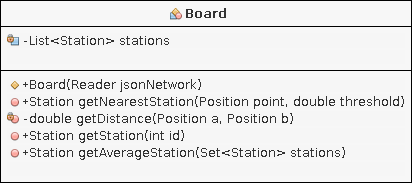
\includegraphics[scale=0.7]{img/uml/board.png}   
                \caption{Board UML-Klassendiagramm}
            \end{figure}


        \subsubsection{Station}
            \begin{table}[H]
                \caption{Klasse Station}
                \begin{tabular}{p{2.5cm}  p{9.5cm}} 
                    \hline
                    \textbf{Eigenschaft} & \textbf{Beschreibung}\\
                    \hline
                    Name & Station\\
                    Ort & Quellpaket \textit{logic.board}\\
                    \hline
                    Zweck &
                    Repräsentiert eine Station und somit einen Knotenpunkt im Netz.
                    \\
                    \hline
                    Struktur &
                    \begin{itemize}
                        \itemsep0em
                        \item Hält vier \textit{Sets} von \textit{Stations} die jeweils ein Verbindung zu anderen Stationen repräsentieren
                        \item Besitzt ein \textit{Occupied}-Flag welches aussagt, ob die Station besetzt ist oder nicht
                        \item Gibt über die \textit{getSurroundingStations}-Methode alle umliegenden Stationen zurück
                        \item Gibt über die \textit{getStationsReachableBy}-Methode alle Stationen wieder, die über das übergebene Ticket erreichbar sind
                        \item Gibt über die \textit{getTicketsToReachableStation}-methode das Ticket wieder, welches benötigt wird um die Station zu erreichen
                    \end{itemize}
                    \\
                    \hline
                \end{tabular}
            \end{table}

            \begin{figure}[H]
                \centering
                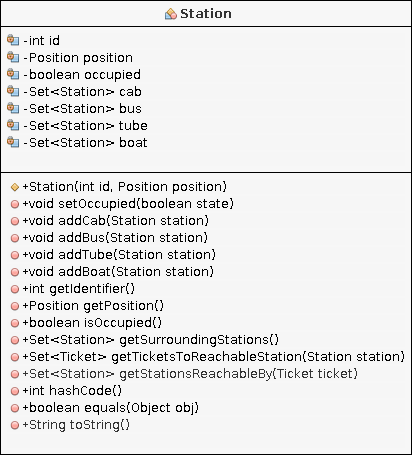
\includegraphics[scale=0.7]{img/uml/station.png}   
                \caption{Station UML-Klassendiagramm}
            \end{figure}



        \subsubsection{Position}
            \begin{table}[H]
                \caption{Klasse Position}
                \begin{tabular}{p{2.5cm}  p{9.5cm}} 
                    \hline
                    \textbf{Eigenschaft} & \textbf{Beschreibung}\\
                    \hline
                    Name & Position\\
                    Ort & Quellpaket \textit{logic.board}\\
                    \hline
                    Zweck &
                    Eine Hilfsklasse die zweidimensionale Koordinaten abbildet.
                    Wird benötigt um die Position der Stationen zu speichern.
                    \\
                    \hline
                    Struktur &
                    \begin{itemize}
                        \itemsep0em
                        \item Hält jeweils den X und den Y Anteil einer Position
                        \item bietet Funktionen die X und Y Werte auszulesen
                    \end{itemize}
                    \\
                    \hline
                \end{tabular}
            \end{table}

            \begin{figure}[H]
                \centering
                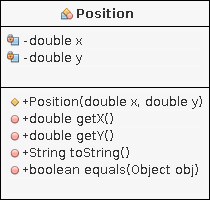
\includegraphics[scale=0.7]{img/uml/position.png}   
                \caption{Position UML-Klassendiagramm}
            \end{figure}